\chapter{Tabellen}
\section{Normale Tabellen}

\begin{figure}
    \caption{Tabelle}
    \label{Kleine Test Tabelle}
    % Label
    % \label{tab:tabular_table}
    \begin{tabular}{|l|c|r|}
        \hline
        \textbf{Spalte 1}                  & \textbf{Spalte 2} & \textbf{Spalte 3} \\
        \hline
        Inhalt 1                           & Inhalt 2          & Inhalt 3          \\
        \multicolumn{2}{|c|}{Zwei Spalten} & InhaltX                               \\
        \hline
    \end{tabular}
\end{figure}


\section{Größere Tabelle}

\begin{tabular}{|l|c|r|p{5cm}|@{ Spalte 5 }|}
    \hline
    left                             & center                      & right        & Mit fester Breite von 5 cm und Zeilenumbruch            \\
    \cline{1-3}
    Spalte 1                         & Spalte 2                    & Spalte 3     & In Spalte 5 \newline steht immer das gleiche            \\
    \hline
    \multicolumn{3}{|c|}{nicht viel} & aber so sind viele Tabellen                                                                          \\
    \cline{4-4}
    Noch                             & eine                        & Zeile        & ohne viel Inhalt -- aber der stand nicht im Vordergrund \\
    \hline
    Eine                             & leere                       & Zeile        & das geht auch                                           \\
                                     &                             &              &                                                         \\
    Sogar                            & zweimal                     &              &                                                         \\
    \hline
                                     &                             &              &                                                         \\
                                     &                             &              &                                                         \\
    Nur                              & die                         & automatische & Spalte ist ein bisschen anders                          \\
    \hline
    Und                              & nochmal                     & mit          & vline \vline auch \vline es komisch \vline aussieht     \\
    \hline
\end{tabular}

\newpage

\section{Tabellen ausrichten}

\lipsum[1-2]

\begin{table}[h]
    \caption{Eine erweiterte tabularx tabelle}

    % \label{tab:tabularx_table}
    \begin{tabularx}{\textwidth}{|X|X|X|}
        \hline
        \textbf{Spalte1}  & \textbf{Spalte2}  & \textbf{Spalte3}  \\
        \hline
        Inhalt Inhalt 1 1 & Inhalt Inhalt 1 2 & Inhalt Inhalt 1 3 \\
        Inhalt Inhalt 2 1 & Inhalt Inhalt 2 2 & Inhalt Inhalt 2 3 \\
        Inhalt Inhalt 3 1 & Inhalt Inhalt 3 2 & Inhalt Inhalt 3 3 \\
        \hline
    \end{tabularx}
\end{table}

\lipsum[1-2]

\lipsum[1-2]

\begin{figure}[h]
    \centering
    \label{tux}
    
\includegraphics[height=2cm]{assets/icon.png}
    \caption{Das Linux Maskottchen}
\end{figure}

\lipsum[1-2]

\ldots wie in Abbildung \ref{tux} gezeigt, \ldots
Hier ist jemand: \cite{einstein} \cite{knuth-fa}
% Zeigt alles im Verzeichnis an
\nocite{*}

\color{blue}
\href{https://mik-mueller.de}{Meine Website}
\color{black}

\chapter{Formeln}
\section{Inline}
Hier ist die Formel $f_{(x)}=m \cdot x + b$ für eine Lineare Funktion
\section{Block}
$$f_{(x)}=ax^3+bx^2+cx$$
Oder
\begin{equation}
    f(x) = m \cdot x + b
    \label{Lineare Funktion}
\end{equation}

\section{Labels}
\begin{equation}
    \label{eq:einstein}
    E = mc^2
\end{equation}

Oder um eine \hyperref[eq:einstein]{Formel} referenzieren zu können.

\section{Formel Array}

\begin{eqnarray}
    E &=& mc^2 \qquad \qquad \text{sinnvolle Beschreibung.} \\
    \Leftrightarrow c^2 &=& \frac{E}{m} \\
    c &=& \sqrt{\frac{E}{m}}
\end{eqnarray}

Formeln \footnote{Macht Mathe Zeug} sind toll.


Es ist 5 $\degree$ Celsius.

\section{Rechnungen}
\begin{align*}
     &                 & E   & = mc^2               &  & |\, :m      \\
     & \Leftrightarrow & c^2 & = \frac{E}{m}        &  & |\, \sqrt{} \\
     & \Leftrightarrow & c   & = \sqrt{\frac{E}{m}}                  \\
\end{align*}

\begin{align*}
     & \Leftrightarrow & f(x)=mx+b &  & | \cdot 4
\end{align*}

\chapter{Minipages}

Hier sind  \hyperref[fig:kabel]{Kabel} und \hyperref[fig:server]{Server} zusehen.


\begin{figure}[h]
    \begin{minipage}{.42\linewidth}
        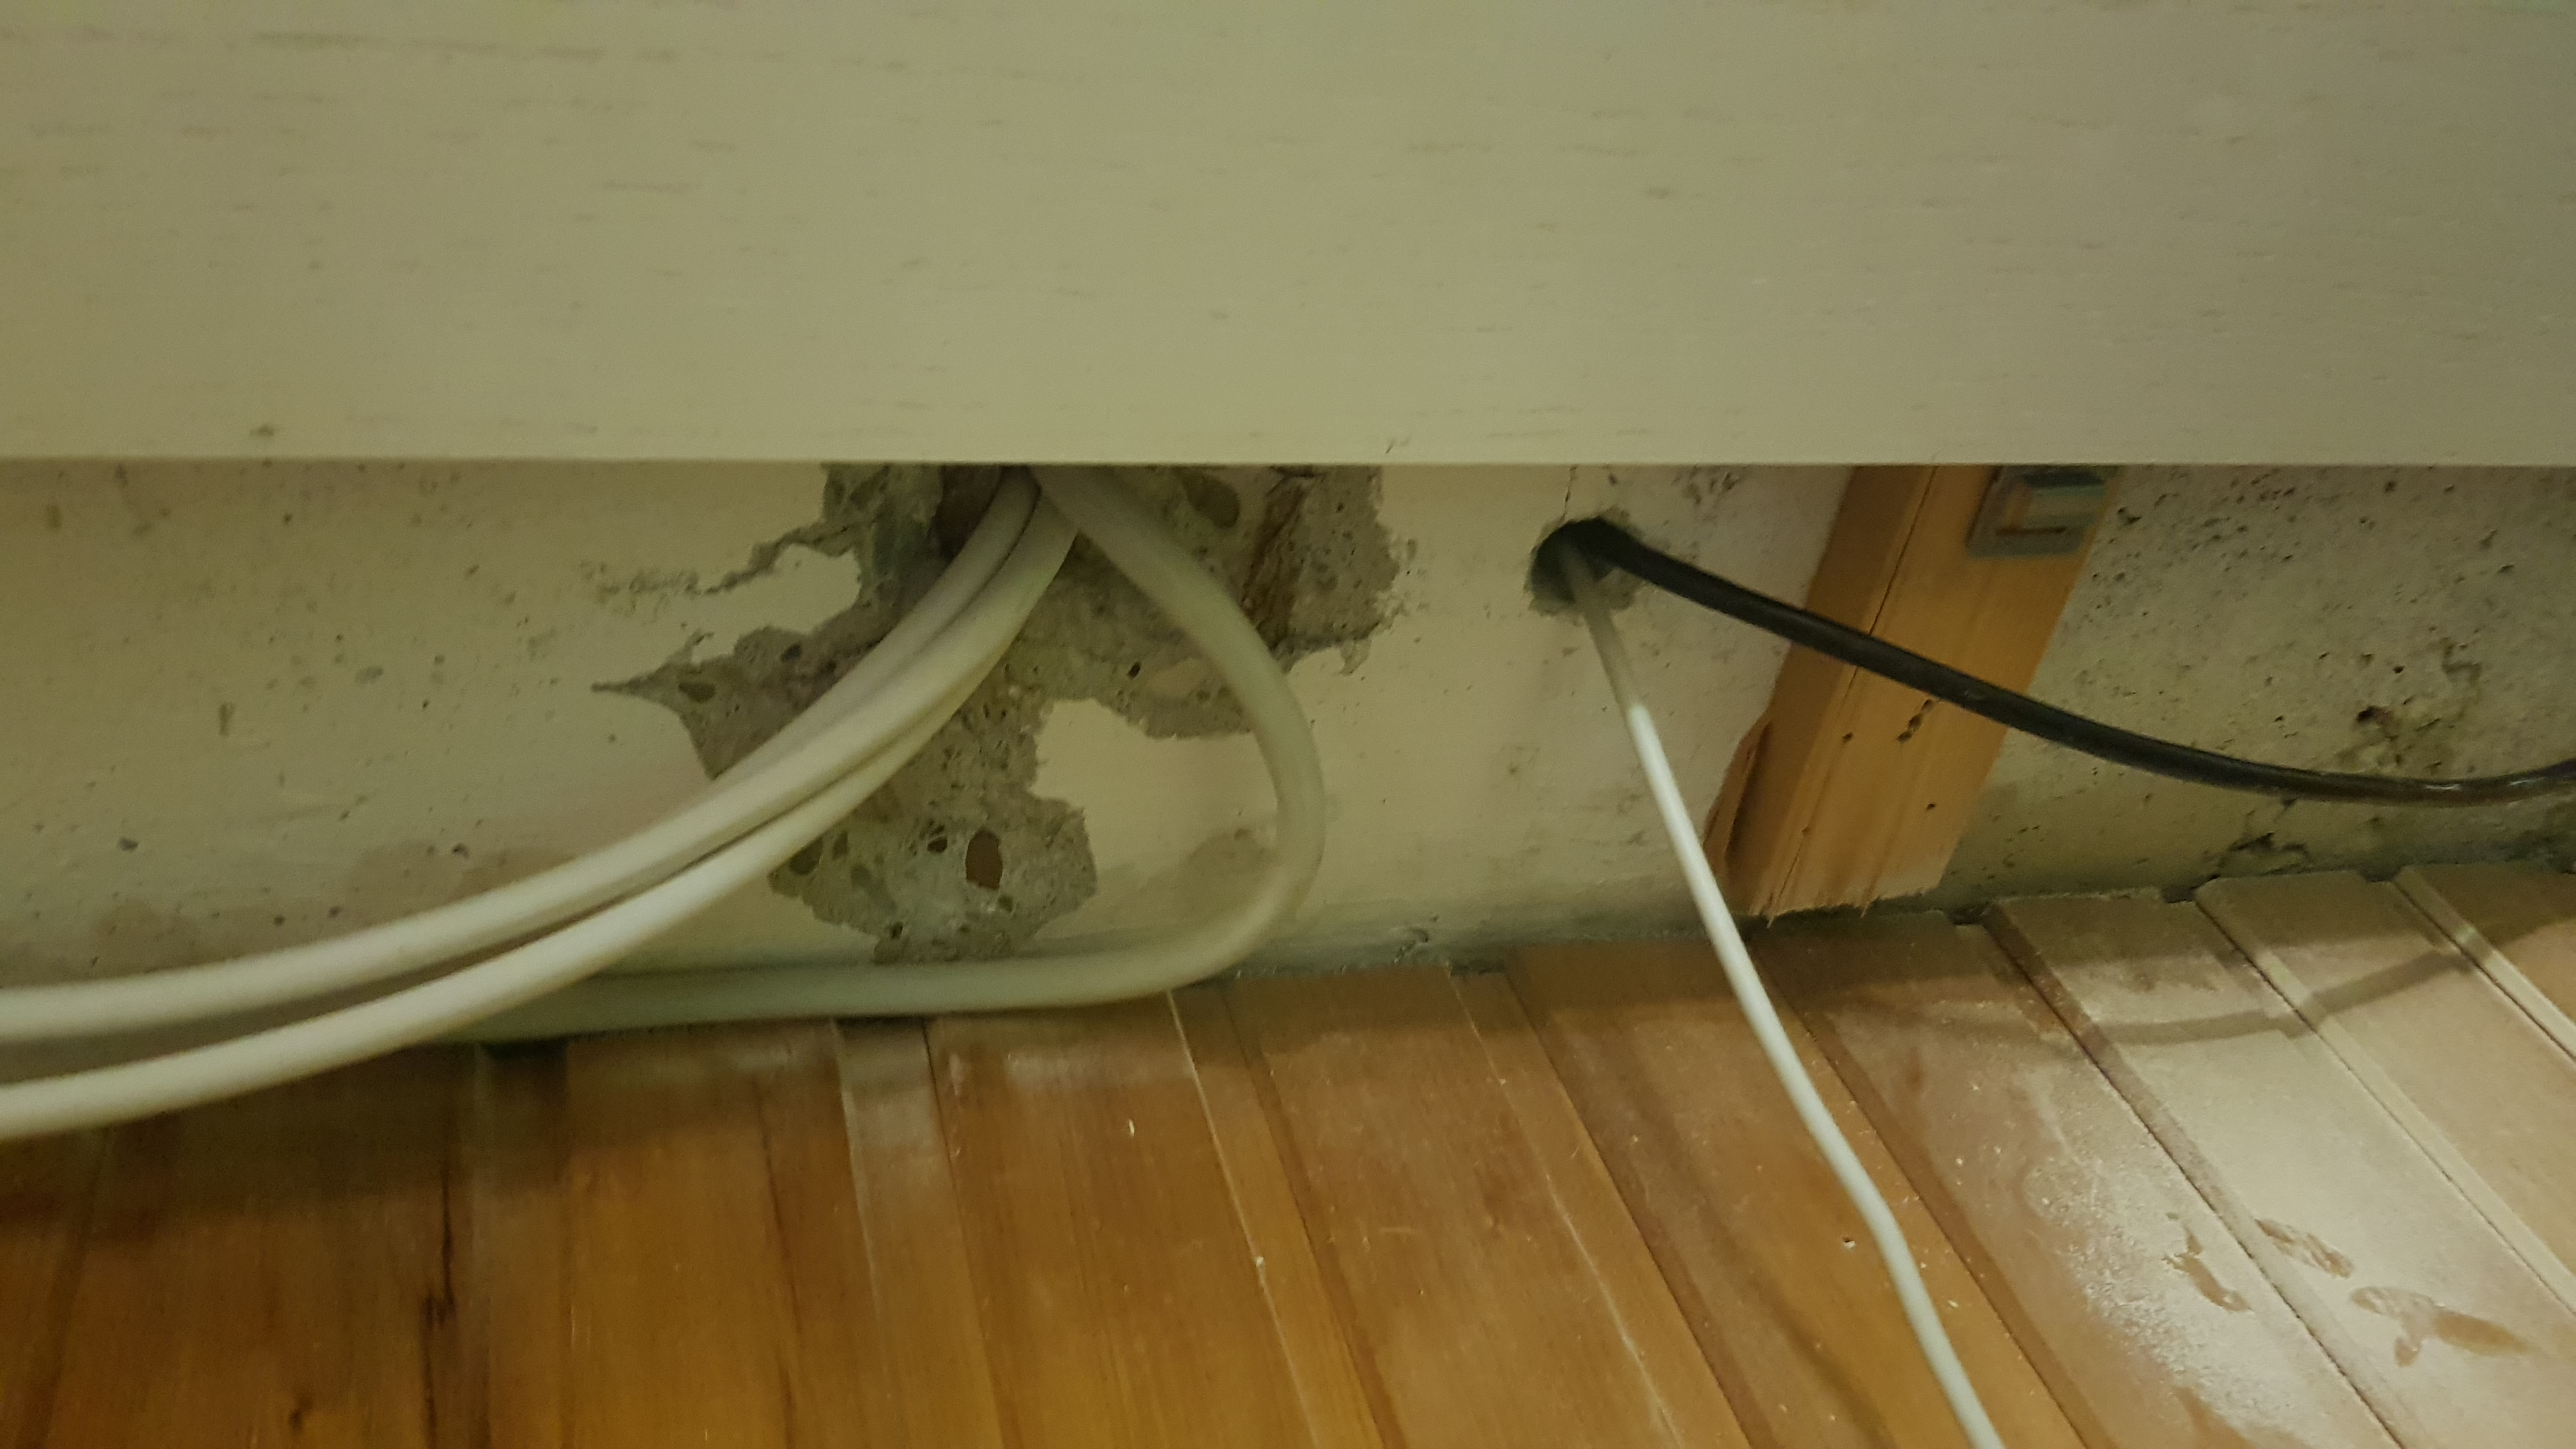
\includegraphics[width=\linewidth]{assets/1.jpg}
        \caption{Kabel}
        \label{fig:kabel}
    \end{minipage}
    \hfill
    \begin{minipage}{.42\linewidth}
        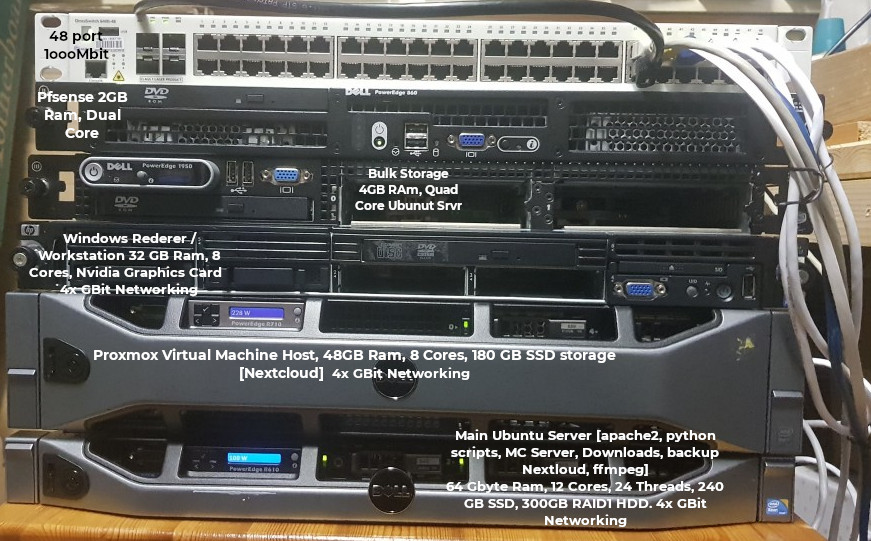
\includegraphics[width=\linewidth]{assets/2.jpg}
        \caption{Server}
        \label{fig:server}
    \end{minipage}
    \centering
    \fcolorbox{red}{gray} {
        \begin{minipage}{.42\linewidth}
            
\includegraphics[width=\linewidth]{assets/icon.png}
            \caption{Tux}
            \label{fig:tux}
            % TODO mach das
        \end{minipage}
    }
\end{figure}

\chapter{Farben}
\color{blue}
\lipsum[1-2]
\color{black}

\textcolor{red}{Roter Text} Text armer Text

\chapter{Side Captions}

\lipsum[1-2]
\begin{figure}[h]
    \caption{This is a caption}
    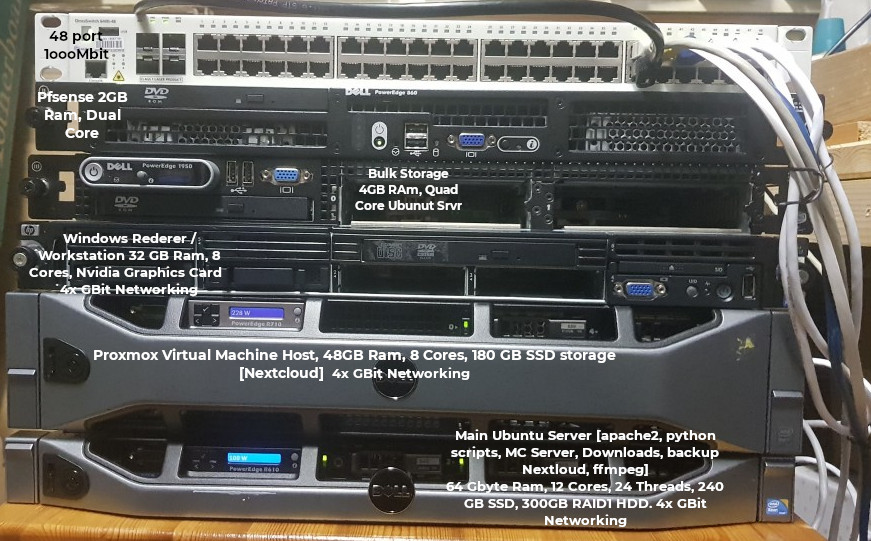
\includegraphics[width=4cm]{assets/2.jpg}
\end{figure}
\lipsum[1-2]


\lipsum[1-2]
\begin{wrapfigure}{r}[0cm]{2cm}
    \raggedleft
    \caption{\label{TestGrafik}}
    
\includegraphics[width=2cm]{assets/icon.png}
\end{wrapfigure}
\lipsum[1-2]


% \begin{SCfigure}
%     \caption{This is a caption}
%     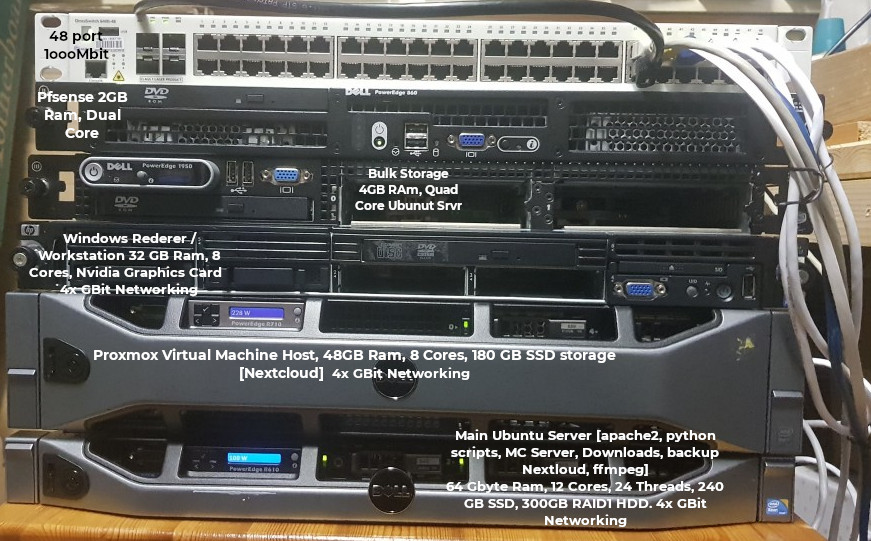
\includegraphics[width=4cm]{assets/2.jpg}
% \end{SCfigure}

$E = mc^2$ \cite{einstein}